\section{Hardware}
\label{sec:chapterexample}

\subsection{Hardware System Übersicht}
Das System wird Hardwareseitig hauptsächlich in zwei Teile unterteilt. Der Server, die zentrale Einheit und die Aussensprechstelle.
\\
Die \cref{fig:hwoverview} bietet ein Überblick über die verschiedene Hardware Komponenten die zusammenarbeiten werden.
\begin{figure}[htb!]
	\begin{center}
		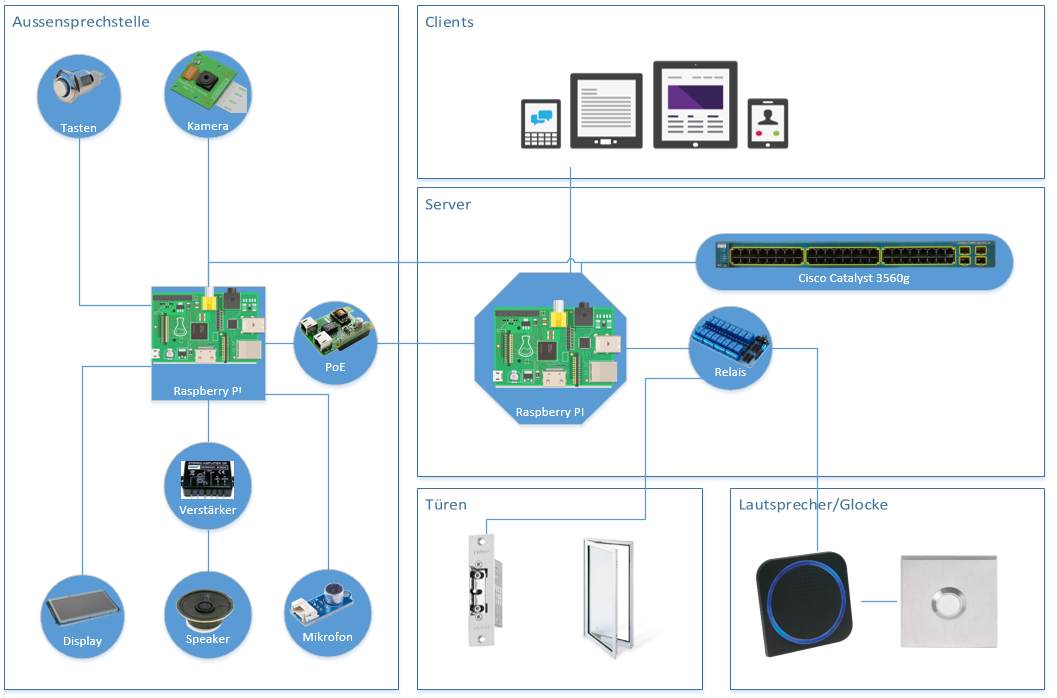
\includegraphics[width=1\textwidth]{hwoverview}
		\caption[Hardware Ecosystem]{Hardware Ecosystem}
		\label{fig:hwoverview}
	\end{center}
\end{figure}
\subsection{Komponenten}
Die \cref{tbl:SrvHW} und die \cref{tbl:DoorHW} zeigen die benötigten HW-Komponenten, welchen an die jeweilige Stellen benötigt werden.
\\
Um den Überblick über die Kosten aller Hardware-Komponenten zu behalten, sind hier auch die Preisen aufgelistet. Wichtig hier ist sicherzustellen, dass die gesamten Hardwarekosten diejenigen der von der Konkurrenz angebotenen Produkte nicht übersteigen.
\\
Die Preise können natürlich leicht abweichen da es sich um Standardkomponenten handelt und die Preise sich schnell ändern. Die Summen sind mehr als Kostenschätzung zu betrachten.

\begin{table}[]
	\centering
	\label{my-label}
	\begin{tabular}{l|ll}
		\multicolumn{1}{r|}{} \textbf{Anzahl} & \textbf{Komponent} \hspace{180pt} & \textbf{Preis} 	\\ \hline
		1	&	Raspberry Pi 3 Model B						& 50.-				\\ \hline
		1	&	Raspberry Gehäuse und Netzteil				& 25.-			\\ \hline
		2	&	8-Kanal Relais Modul						& 15.-			\\ \hline
		1	&	\textit{Kleinmaterial}						& 15.-			\\ \hline
		\textbf{Total}	&									& \textbf{140.-}			\\ \hline
	\end{tabular}
	\caption{Server HW Komponenten}
	\label{tbl:SrvHW}
\end{table}

\begin{table}[]
	\centering
	\label{my-label}
	\begin{tabular}{l|ll}
		\multicolumn{1}{r|}{} \textbf{Anzahl} & \textbf{Komponent} \hspace{180pt} & \textbf{Preis} 	\\ \hline
		1	&	Raspberry Pi 3 Model B		   				& 50.-			\\ \hline
		1	&	4" Bildschirm								& 64.-			\\ \hline
		1	&	Raspberry Kamera							& 59.-			\\ \hline
		1	&	PoE Adapter									& 50.-			\\ \hline
		3	&	Schalter									& 25.-			\\ \hline
		1	&	Mikrophon									& 12.-			\\ \hline
		1	&	Lautsprecher								& 9.-			\\ \hline
		1	&	Audio Verstärker							& 10.-			\\ \hline
		1	&	\textit{Kleinmaterial / Gehäuse}			& 50.-			\\ \hline
		\textbf{Total}	&									& \textbf{329.-}			\\ \hline
	\end{tabular}
	\caption{Aussensprechstelle HW Komponenten}
	\label{tbl:DoorHW}
\end{table}


\subsection{Server}
\label{sec:chapterexample}

Der Server wird mit einem Relay-Board verbunden. Diese wird die Gongs und die Türöffner bedienen. An dieser Stelle ist die Hardware-Konfiguration sehr einfach. Mit der jetzige Hardwarekonfiguration könnten bis auf 8 Wohnungen und 8 Aussensprechstellen angeschlossen werden. Die \cref{fig:pipins} und die \cref{fig:boardpins} zeigen die PIN-Belegung auf den Pi und auf dem Relay-Board. Die \cref{tbl:pinroutes} zeigt wie die verschiedene Pins miteinander angeschlossen werden.

\begin{figure}[htb!]
	\begin{center}
		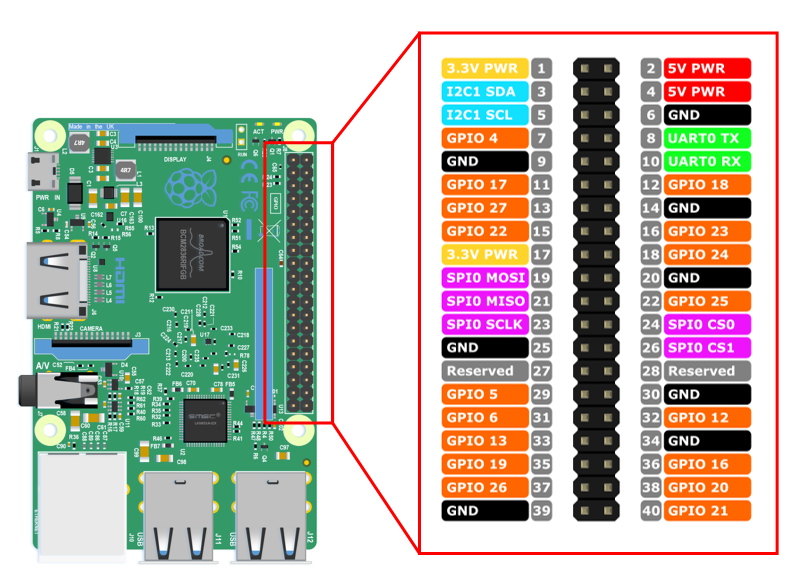
\includegraphics[width=0.8\textwidth]{pipins}
		\caption[EthernetPinbelegung]{Pinbelegung für die Aussensprechstellen}
		\label{fig:pipins}
	\end{center}
\end{figure}

\begin{figure}[htb!]
	\begin{center}
		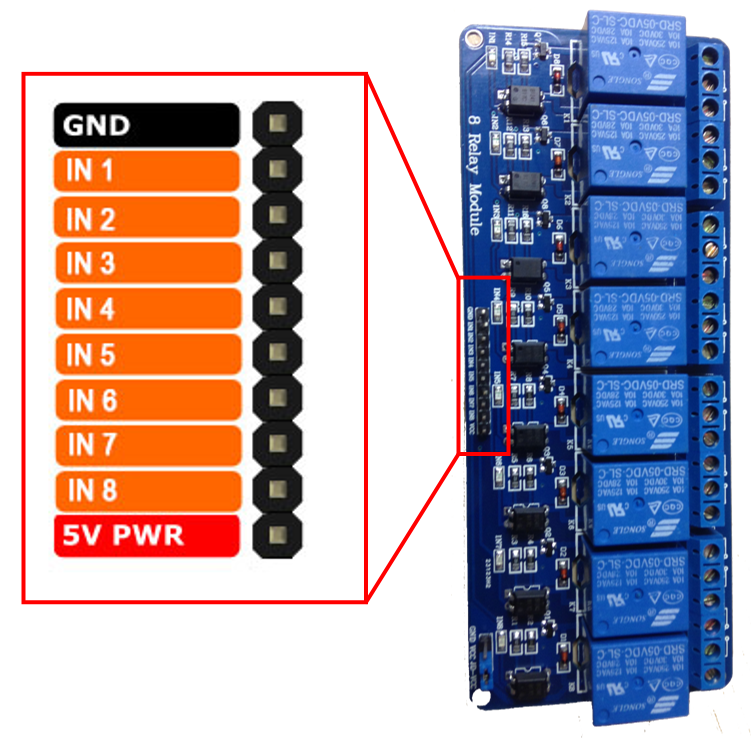
\includegraphics[width=0.55\textwidth]{boardpins}
		\caption[EthernetPinbelegung]{Pinbelegung für das Relais-Modul}
		\label{fig:boardpins}
	\end{center}
\end{figure}

\begin{table}[]
	\centering
	\label{my-label}
	\begin{tabular}{l|ll}
		\multicolumn{1}{r|}{} \textbf{Pi GPIO (PIN)} & \textbf{Relais IN (Board Nr)} & \textbf{Funktion}  \hspace{60pt}	\\ \hline
		GPIO4 (7)	&	IN1 (1)			& Gong WG.1			\\ \hline
		GPIO17 (11)	&	IN2 (1)			& Gong WG.2			\\ \hline
		GPIO27 (13)	&	IN3 (1)			& Gong WG.3			\\ \hline
		GPIO22 (15)	&	IN4 (1)			& Gong WG.4			\\ \hline
		GPIO5 (29)	&	IN5 (1)			& Gong WG.5			\\ \hline
		GPIO6 (31)	&	IN6 (1)			& Gong WG.6			\\ \hline
		GPIO13 (33)	&	IN7 (1)			& Gong WG.7			\\ \hline
		GPIO19 (35)	&	IN8 (1)			& Gong WG.8			\\ \hline
		GPIO18 (12)	&	IN1 (2)			& Türöffner Türe 1			\\ \hline
		GPIO23 (16)	&	IN2 (2)			& Türöffner Türe 2			\\ \hline
		GPIO24 (18)	&	IN3 (2)			& Türöffner Türe 3			\\ \hline
		GPIO25 (22)	&	IN4 (2)			& Türöffner Türe 4			\\ \hline
		GPIO12 (32)	&	IN5 (2)			& Türöffner Türe 5			\\ \hline
		GPIO16 (36)	&	IN6 (2)			& Türöffner Türe 6			\\ \hline
		GPIO20 (38)	&	IN7 (2)			& Türöffner Türe 7			\\ \hline
		GPIO21 (40)	&	IN8 (2)			& Türöffner Türe 8			\\ \hline
	\end{tabular}
	\caption{PIN-Zuweisung zwischen den Server und die Relais Module}
	\label{tbl:pinroutes}
\end{table}


\subsection{Aussensprechstelle}
\label{sec:chapterexample}

Bei der Aussensprechstelle wird auch eine Raspberry Pi eingesetzt. Hier sind mehrere Zusatzkomponenten notwendig. Die Speisung an dieser stelle erfolgt nur über PoE, aus diesem Grund ist PoE-Splitter vorhanden.
\\
Für die Audiowiedergabe ist ein kleines Lautsprecher und ein Verstärker nötig. Die Chinch-Anschluss der Raspberry Pi hat eine viel zu kleine innere Widerstand um direkt ein solches Lautsprecher anschliessen zu können. Die Hauptproblematik nun besteht darin, dass die Massen des Raspberry Pi, der Verstärker und des Audio-Interface alle zusammen gekoppelt sind. Das führt zu Brunschleifen die wiederum Störsignale auf dem Audio-Ausgang erzeugen. Um das zu vermeiden ist eine Massentrennfilter an dieser Stelle notwendig. Diese Problematik wird im ein eigenes Kapitel genauer erläutert.
Die drei Schalter, die für die Bedienung der Aussensprechstelle notwendig sind werden an die GPIOs der Raspberry PI angeschlossen. Die \cref{tbl:pinroutesdoor} zeigt die PIN-Zuweisung.
\begin{table}[]
	\centering
	\label{my-label}
	\begin{tabular}{l|ll}
		\multicolumn{1}{r|}{} \textbf{Pi GPIO (PIN)} & \textbf{Schalter} & \textbf{Funktion} \hspace{60pt}	\\ \hline
		GPIO16 (36)	&	Schalter Links		&	Nach Links Scrollen	\\ \hline
		GPIO20 (38)	&	Schalter Mitte		&	Glocke läuten		\\ \hline
		GPIO21 (40)	&	Schalter Rechts		&	Nach Rechts Scrollen		\\ \hline
	\end{tabular}
	\caption{PIN-Zuweisung zwischen den Raspberry PI und die Schalter}
	\label{tbl:pinroutesdoor}
\end{table}


\subsection{Power over Ethernet}
\label{sec:poe}
Moderne Hausalte werden meistens mit ethernet Verkabelung verlegt. Ziel des Aussensprechstelle ist die Installationskosten zu senken und die Montage zu vereinfachen. Drei Anschlusse werden von den Aussensprechstelle benötigt um sein Ziel zu erreichen und zwar Strom, Internetverbindung und eine Leitung der den Türöffner betätigt. Alle diese Fünktionalität können in einem Kat 7 Ethernet Kabel zusammengeführt werden. 
\\
Cisco Catalyst 3560g welcher für den PoE Stromversorgung zuständigt ist verwendet das Phantomspeisung oder Mode A. Das heisst dass die mit Datenübertragung belegten Adern mit der Stromversorgung überlagert werden. Diese ist möglich da Elektrizität eine niedrige Frequenz von 60 Hz hat und Datenübertragungen im bereich 10-100MHz liegen.

\begin{figure}[htb!]
	\begin{center}
		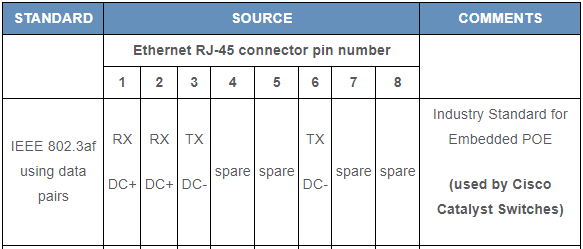
\includegraphics[width=0.89\textwidth]{CatalystPoEpinouts}
		\caption[Catalyst Pinouts]{Catalyst 3560g PoE Pinbelegung}
		\label{fig:catalystPinouts}
	\end{center}
\end{figure}

Wie im Abbild nr.5!!? dargestellt werden die Adern 7 und 8 dazu verwendet um der Türöffner zu betätigen. Aus den 3 verbliebenden Adernpaare kann maximal die Ethernet Kategorie 100BASE-T erreicht werden. Da aber WebRTC eine erhebliche kleinere Bandbreite in Anspruch nimmt, stellt für die Aussensprechtellen kein Hinderniss dar.

\begin{figure}[htb!]
	\begin{center}
		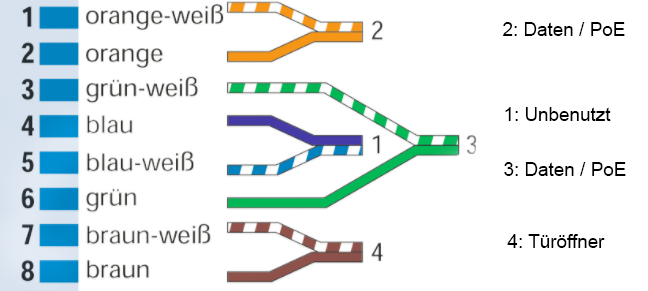
\includegraphics[width=0.89\textwidth]{EthernetPinbelegung}
		\caption[EthernetPinbelegung]{Cat. 7 Ethernet Pinbelegung für die Aussensprechstellen}
		\label{fig:catalystPinouts}
	\end{center}
\end{figure}


\newpage